\documentclass[11pt]{beamer}
\usepackage{mmacells}
\usetheme{AnnArbor}
\setbeamercolor{normal text}{bg=black!10}
\begin{document}
\title{Design of Integrated Microrobotic Fish}
\subtitle{Presentation 3 - Physical Model (Complete) \& COMSOL Simulation}
\author{Yihua Liu}
\institute{UM-SJTU Joint Institute}
\date{March 9, 2021}
\begin{frame}
    \titlepage
\end{frame}
\section{Antecedent}
\begin{frame}[fragile]{Antecedent}{Total Impedance $Z$}
        \begin{mmaCell}{Input}
            R=\mmaFrac{Pi*x*(\mmaSqrt{k}+\mmaFrac{1}{\mmaSqrt{k}})}{2\mmaUnd{\(\pmb{\sigma}\)}*\mmaUnd{\(\pmb{\delta}\)x}};
            \mmaSub{C}{DL}=\mmaFrac{\mmaUnd{\(\pmb{\epsilon}\)}*\mmaUnd{\(\pmb{\delta}\)x}*\mmaSqrt{k}}{\mmaSub{\mmaUnd{\(\pmb{\lambda}\)}}{D}};
            \mmaSub{C}{DS}=\mmaFrac{\mmaUnd{\(\pmb{\epsilon}\)}*\mmaUnd{\(\pmb{\delta}\)x}}{\mmaSqrt{k}*\mmaSub{\mmaUnd{\(\pmb{\lambda}\)}}{D}};
            Zx=R+\mmaFrac{1}{I*\mmaUnd{\(\pmb{\omega}\)}*\mmaSub{C}{DL}}+\mmaFrac{1}{I*\mmaUnd{\(\pmb{\omega}\)}*\mmaSub{C}{DS}}
        \end{mmaCell}
        \begin{mmaCell}[addtoindex=3]{Output}
            \mmaFrac{(\mmaFrac{1}{\mmaSqrt{k}}+\mmaSqrt{k}) \(\pi\) x}{2\(\delta\)x \(\sigma\)}-\mmaFrac{i\mmaSub{\(\lambda\)}{D}}{\mmaSqrt{k} \(\delta\)x\(\epsilon \omega\)}-\mmaFrac{i \mmaSqrt{k} \mmaSub{\(\lambda\)}{D}}{\(\delta\)x \(\epsilon \omega\)}
        \end{mmaCell}
        \begin{mmaCell}[addtoindex=5]{Input}
            Simplify[Zx]
        \end{mmaCell}
        \begin{mmaCell}{Output}
            \mmaFrac{(1+k) (\(\pi\) x \(\epsilon \omega\)-2 i \(\sigma\)\mmaSub{\(\lambda\)}{D})}{2 \mmaSqrt{k} \(\delta\)x \(\epsilon \sigma\omega\)}
        \end{mmaCell}
    % \begin{columns}[onlytextwidth]
        % \begin{column}{0.4\textwidth}
        % \end{column}
        % \begin{column}{0.6\textwidth}
        %     \begin{itemize}
        %         \item The double layers at the electrode surfaces -\textgreater Capacitance\\
        %               The capacitance of the double layer at each end of the tube per unit length of the electrode $C_{DL}$ and at the large electrode $C_{DS}$
        %         \item The bulk water -\textgreater Resistance\\
        %               The resistance of the tube per unit length of electrode $R(x)$
        %     \end{itemize}
        % \end{column}
    % \end{columns}
\end{frame}
\begin{frame}[fragile]{Antecedent}{Total Impedance $Z$}
    Remind the formula given in the article
    \[Z=\frac{\pi\left(\sqrt{k}+\frac{1}{\sqrt{k}}\right)}{2l\sigma}\frac{\ln{A}-i\theta}{(\ln{A})^2+\theta^2}\]
    where
    \[A=\frac{\sqrt{\left[\left(2\lambda_D\sigma\right)^2+(\omega\varepsilon\pi)^2+x_{min}x_{max}\right]^2+\left[2\lambda_D\sigma\omega\varepsilon\pi\left(x_{max}-x_{min}\right)\right]^2}}{\left(2\lambda_D\sigma\right)^2+(\omega\varepsilon\pi x_{min})^2}\]
    and\\
    \[\theta=\arctan{\frac{2\lambda_D\sigma\omega\varepsilon\pi\left(x_{max}-x_{min}\right)}{\left(2\lambda_D\sigma\right)^2+(\omega\varepsilon\pi)^2x_{min}x_{max}}}\]
    The author made a mistake of the parameter $A$. The correct formula is
\end{frame}
\begin{frame}{Antecedent}{Total Impedance $Z$}
    \includegraphics[width=0.9\textwidth]{1.eps}
\end{frame}
\begin{frame}{Antecedent}{Total Impedance $Z$}
    \includegraphics[width=1\textwidth]{2.eps}
\end{frame}
\begin{frame}{Antecedent}{Total Impedance $Z$}
    Here we restore the resistance to three-dimensional by dividing by the total length of the electrodes in the cell $l=23.5$ cm.\\
    From the results above, we found that the corrected value of $\mathrm{Re}\{Z\}$ is in the range of 0.1 k$\Omega$ - 1 k$\Omega$ but differs from the value in FIG. 7. of the article.
\end{frame}
\end{document}